% !TEX TS-program = pdflatex
% !TEX root = ../LightMicroRep.tex

%************************************************
\chapter{Airyscan}
\label{chp:Airyscan}
%************************************************
%\numberwithin{figure}{section}
%----------------------------------------------------------------------------------------
%	INTRODUCTION
%----------------------------------------------------------------------------------------

\section{Introduction}

\paragraph{Aim}To study the features of Airyscan technology and compare with conventional confocal techniques.
\\

The Airyscan method is similar to conventional confocal Laser Scanning Microscopy (LSM) , however in this method, instead of using a physical pinhole, a special detector is utilized for the same purpose of confocal LSM.  
This Airyscan detector is a 32-channel gallium arsenide phosphide photomultiplier tube (GaAsP-PMT) area detector that collects a pinhole-plane image at every scan position \cite{Huff2015}. 

\begin{figure}[h!]
\centering
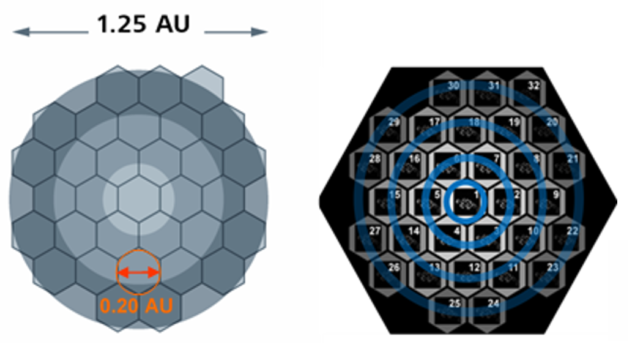
\includegraphics[width=.5\columnwidth]{Exp_6_Airyscan/Figures/airyscan_ed}
\caption{Airyscan detector. Image adapted from: \href{https://cif.unil.ch/the-airyscan-system-for-improved-confocal-resolution/}{\textit{https://cif.unil.ch/the-airyscan-system-for-improved-confocal-resolution/}}. Accessed: 02/01/2021.} 
\label{fig:airydet}
\end{figure}

This special detector (Fig.~\ref{fig:airydet}), which organized the area detector in a honeycomb-like structure (each detector acting as an individual pinhole with diameter 0.2 AU), and positioned in the conjugate focal plane (like the pinhole on conventional confocal microscopy) made it possible to collect more light (equivalent to a pinhole opened to 1.25 AU), and hence allows for an enhancement of resolution by the factor of 1.7 x and SNR by 4–8 times \cite{Bergter2016} in comparison to conventional confocal technique, where the downside to using a pinhole with a diameter less than 1 AU is the dramatic decrease in signal reaching the detector (95\% loss at 0.2 AU) \cite{Huff2015}.

%----------------------------------------------------------------------------------------
%	METHODS
%----------------------------------------------------------------------------------------

\section{Methods}
The specimens used for this experiment are: 
\begin{itemize}
\item Blowfly salivary gland. Actin labelled by AlexaFluor488-Phalloidin (green) and microtubules/septate junctions by anti-Na,K-ATPase ($\alpha$5) / goat anti-mouse-IgG, AlexaFluor568-conjugated (magenta).
\item AX2 line of \textit{Dictyostelium discoideum} from expansion microscopy experiment. CP91 (centrosome core) labelled by AlexaFluor568 (magenta) and CP224 (centrosome corona) by AlexaFluor488 (green). 
\end{itemize}

The device used in this experiment is Zeiss LSM-880 with an Airyscan detection unit, the objectives are 40$\times$/1.2 lmm for the salivary gland and 63$\times$/1.3 Oil immersion lens for the AX2 specimen. 

The following was performed:
\begin{enumerate}
\item Airyscan acquisition
\item LSM acquisition with pinhole opening larger than 1 AU
\item LSM acquisition with twice the the optimal number of pixels in the lateral dimension and half optimal distance in the axial dimension (then proceed with deconvolution)
\item Airyscan acquisition without module with pinhole size of 0.2 AU
\end{enumerate}

The AX2 specimen was imaged only by Airyscan and LSM. The \textit{Elodea} specimen listed for this experiment was dead and hence no data is available. 


%----------------------------------------------------------------------------------------
%	RESULTS AND DISCUSSION
%----------------------------------------------------------------------------------------
\section{Results and Discussion}

\begin{figure}[h!]
\centering
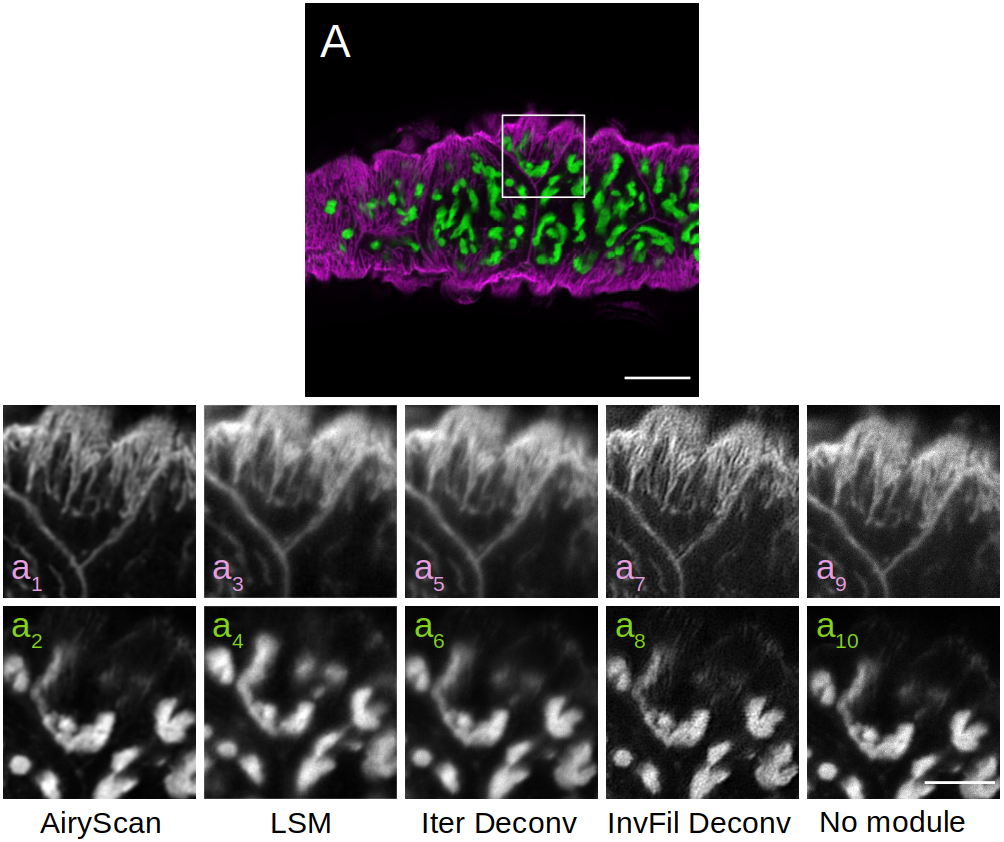
\includegraphics[width=\columnwidth]{Exp_6_Airyscan/Figures/BlowSl}
\caption{A: Airyscan of a blowfly salivary gland, white square marks the magnified area. 
All images are shown at an approximately similar optical section of a z-stack. 
Top row (odd index) is the basolateral membrane labelled by anti-mouse-AlexaFluor568, bottom row (even index) is Actin, labelled by AlexaFluor488-Phalloidin. 
Objective lens: 40$\times$/1.2 lmm glycerin immersion. 
Scalebar on original image is 10 $\mu$m, on the zoomed in image is 5 $\mu$m.}
\label{fig:bloair}
\end{figure}

Fig.~\ref{fig:bloair} shows the resulting images of the salivary gland of a blowfly obtained using the previously mentioned methods. 
It can be seen here that the basolateral folds (apical membrane) can be seen better with the Airyscan than with LSM (Fig.~\ref{fig:bloair}~a$_{1}$\&a$_{3}$). 
This is due to oversampling compared to the Nyquist criterion. 
This is also fairly observable by the blurriness of image Fig.~\ref{fig:bloair}~a$_{4}$ when it is quite clear in comparatively in image Fig.~\ref{fig:bloair}~a$_{2}$. 

The constrained iterative deconvolution algorithm employed seem to improve the LSM imaging results (Fig.~\ref{fig:bloair}~a$_{5}$-a$_{7}$), but not quite to the degree of sharpness of Fig.~\ref{fig:bloair}~a$_{1}$. 
Another voluntary deconvolution method that was employed was inverse filter. 
This method does not perform as well as the previous method and seem to even introduce artifacts in the form of graininess, also evident in Fig.~\ref{fig:bloair}~a$_{8}$. 

The removal of the Airyscan module (Fig.~\ref{fig:bloair}~a$_{9}$\&a$_{10}$) warrants the compensation of reducing the pinhole size to 0.2 AU. 
This seem to result in an image that is in detail shows an increasing degree of blurriness/noise than the ones obtained with the module. 
This can be, for the most part, observed in the magenta (AlexaFluor568) channel. 
However the sharpness is still better than LSM with pinhole opening of 1 AU. 
This can also be seen in Fig.~\ref{fig:bloair}~a$_{10}$ in which the image still show a fairly sharp structures of the actins in comparison to Fig.~\ref{fig:bloair}~a$_{4}$, but not to the degree of Fig.~\ref{fig:bloair}~a$_{2}$.  

The advantage of Airyscan compared to the more traditional LSM can be seen more clearly in the images of AX2 cells. 
Comparing both channels of CP91 and CP224 it is obvious that Airyscan (Fig.~\ref{fig:dicair}~b$_{1}$\&b$_{2}$) gives a much higher resolution image with more readily observable structures and less murked by rough noise that is shown on LSM images. 
The sharpness of the centrosome corona (CP224) is also enhanced in Fig.~\ref{fig:dicair}~b$_{2}$ whereas it is very rough in Fig.~\ref{fig:dicair}~b$_{4}$.

\begin{figure}[h!]
\centering
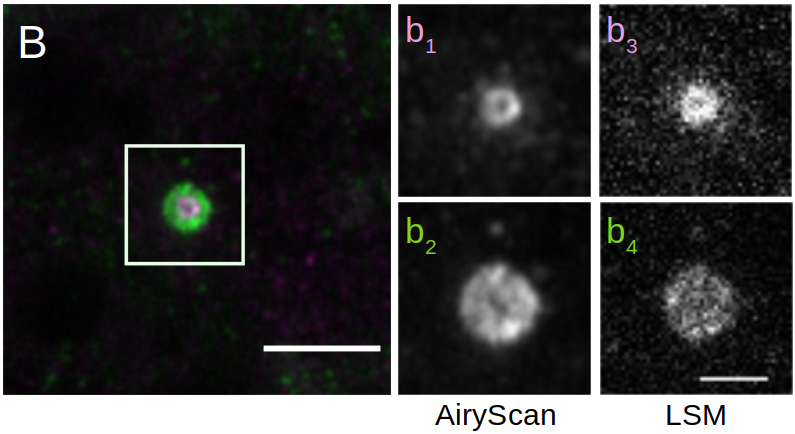
\includegraphics[width=.9\columnwidth]{Exp_6_Airyscan/Figures/DictSl}
\caption{B: Airyscan of AX2, white square marks the magnified area. 
%as the following: b$_{1,2}$: Airyscan, b$_{3,4}$: LSM. 
All images are shown at an approximately similar optical section of a z-stack. 
Top row (odd index) is CP91 labelled by AlexaFluor568, bottom row (even index) is CP224 labelled by AlexaFluor488. 
Objective lens: 63$\times$/1.3 Oil immersion. 
Scalebar on original image is 10 $\mu$m, on the zoomed in image is 1 $\mu$m.} 
\label{fig:dicair}
\end{figure}


%----------------------------------------------------------------------------------------
%	BIBLIOGRAPHY
%----------------------------------------------------------------------------------------

\renewcommand{\refname}{\spacedlowsmallcaps{References}} % For modifying the bibliography heading

%\bibliographystyle{unsrt}

%\bibliography{sample.bib} % The file containing the bibliography
